\documentclass[]{article}
\usepackage{lmodern}
\usepackage{amssymb,amsmath}
\usepackage{ifxetex,ifluatex}
\usepackage{fixltx2e} % provides \textsubscript
\ifnum 0\ifxetex 1\fi\ifluatex 1\fi=0 % if pdftex
  \usepackage[T1]{fontenc}
  \usepackage[utf8]{inputenc}
\else % if luatex or xelatex
  \ifxetex
    \usepackage{mathspec}
  \else
    \usepackage{fontspec}
  \fi
  \defaultfontfeatures{Ligatures=TeX,Scale=MatchLowercase}
\fi
% use upquote if available, for straight quotes in verbatim environments
\IfFileExists{upquote.sty}{\usepackage{upquote}}{}
% use microtype if available
\IfFileExists{microtype.sty}{%
\usepackage{microtype}
\UseMicrotypeSet[protrusion]{basicmath} % disable protrusion for tt fonts
}{}
\usepackage[margin=1in]{geometry}
\usepackage{hyperref}
\hypersetup{unicode=true,
            pdftitle={Presentation and use of our Shiny app !},
            pdfauthor={AKS GROUP},
            pdfborder={0 0 0},
            breaklinks=true}
\urlstyle{same}  % don't use monospace font for urls
\usepackage{graphicx,grffile}
\makeatletter
\def\maxwidth{\ifdim\Gin@nat@width>\linewidth\linewidth\else\Gin@nat@width\fi}
\def\maxheight{\ifdim\Gin@nat@height>\textheight\textheight\else\Gin@nat@height\fi}
\makeatother
% Scale images if necessary, so that they will not overflow the page
% margins by default, and it is still possible to overwrite the defaults
% using explicit options in \includegraphics[width, height, ...]{}
\setkeys{Gin}{width=\maxwidth,height=\maxheight,keepaspectratio}
\IfFileExists{parskip.sty}{%
\usepackage{parskip}
}{% else
\setlength{\parindent}{0pt}
\setlength{\parskip}{6pt plus 2pt minus 1pt}
}
\setlength{\emergencystretch}{3em}  % prevent overfull lines
\providecommand{\tightlist}{%
  \setlength{\itemsep}{0pt}\setlength{\parskip}{0pt}}
\setcounter{secnumdepth}{0}
% Redefines (sub)paragraphs to behave more like sections
\ifx\paragraph\undefined\else
\let\oldparagraph\paragraph
\renewcommand{\paragraph}[1]{\oldparagraph{#1}\mbox{}}
\fi
\ifx\subparagraph\undefined\else
\let\oldsubparagraph\subparagraph
\renewcommand{\subparagraph}[1]{\oldsubparagraph{#1}\mbox{}}
\fi

%%% Use protect on footnotes to avoid problems with footnotes in titles
\let\rmarkdownfootnote\footnote%
\def\footnote{\protect\rmarkdownfootnote}

%%% Change title format to be more compact
\usepackage{titling}

% Create subtitle command for use in maketitle
\providecommand{\subtitle}[1]{
  \posttitle{
    \begin{center}\large#1\end{center}
    }
}

\setlength{\droptitle}{-2em}

  \title{\textbf{Presentation and use of our Shiny app ! }}
    \pretitle{\vspace{\droptitle}\centering\huge}
  \posttitle{\par}
    \author{\emph{AKS GROUP}}
    \preauthor{\centering\large\emph}
  \postauthor{\par}
      \predate{\centering\large\emph}
  \postdate{\par}
    \date{17 novembre, 2019}


\begin{document}
\maketitle

\section{Welcome to our Shiny app !}\label{welcome-to-our-shiny-app}

When you launch the link of our application, you will have the
authentication page. Here, you must enter your username and password and
click on the \textbf{Log In} button. After you are authenticated, you
will have access to the content of the application. Please, make sure
that you are correctly authenticating by clicking on the button at the
top on the right

\includegraphics[width=0.40000cm]{https://raw.githubusercontent.com/Songui/Image/master/Capture.PNG}.
If you see the message connected and your name also, it notifies that
you are well connected and our application will properly work.

The button

\includegraphics[width=0.40000cm]{https://raw.githubusercontent.com/Songui/Image/master/Capture1.PNG}
is the notification button. It is at this level that you have been able
to download this notice via the download button to help you in using
this application.

The menus on the right shows the different steps of our application
(Data, Model, Prediction). We invite you to move forward sequentially.
In other words, follow the steps one by one, because they are all
related to each other. This is to allow the proper operation of this
application and permit to have correct results.

We also want to draw your attention to part of the case ``\emph{Data
description from MLG kaggle page}''. You have the description of the
database which allowed us to realize our demonstrator. Know that you can
reduce this frame or leaving it, according to your desires, allowed by

\includegraphics[width=0.40000cm]{https://raw.githubusercontent.com/Songui/Image/master/Capture2.PNG},
which is on the right side. This saves space on a page and avoids
overloading it. At the bottom of the page, you have the link to visit
our formation website indicated by ``© GROUP AKS - MASTER ESA''. Do not
hesitate to click on this link if you are interested or curious.

\emph{\textbf{Attention: it's a dynamic application, so you'll have to
follow the instructions!}}

\section{Data part}\label{data-part}

By clicking on the Data tab, you will have several steps to follow in
order to have the correct results. Please wait a few seconds, as long as
the data is loaded on the application. You can continue when the
variable \textbf{class} will appear in the \emph{Target Variable box}.
It is the target variable of our database. You are now facing 3 boxes:
Target Variable, Others Variables and Load external data if you want!.\\
\textbf{Target Variable box}\\
Here, you just have to select the target variable. But in our case, it
is defined by default. So, you don't have something to do except click
on the submit button to view the database, the general descriptive
statistics of it via the summary tab and some graphics via the graphics
tab.

The two other boxes that we will explain now should not be touched
unless you are interested after understanding what they are doing.

\textbf{Others Variables}\\
In this box, you can select the variable that you want to eliminate (is
you have) for your modeling and if the variable does not provide any
useful information.\\
\textbf{Load external data if you want!}\\
Given the interactivity of our application, you have the opportunity to
work on other databases than the one we are working on.At this level,
you must select the type of file you want to enter and download it.
Then, you have to specify the characteristics of your file concerning
the delimiter, the decimal type and whether the first line refers to
variable names or not (if that is the case, tick the header button
otherwise leave empty). At the end, you must submit this via the submit
button and you will see your database and statistics. Be careful to
select your target variable in the Target Variable Box at this time and
make sure that it is in a binary form (0 or 1). Finally, you will have
this interface :

\begin{figure}
\centering
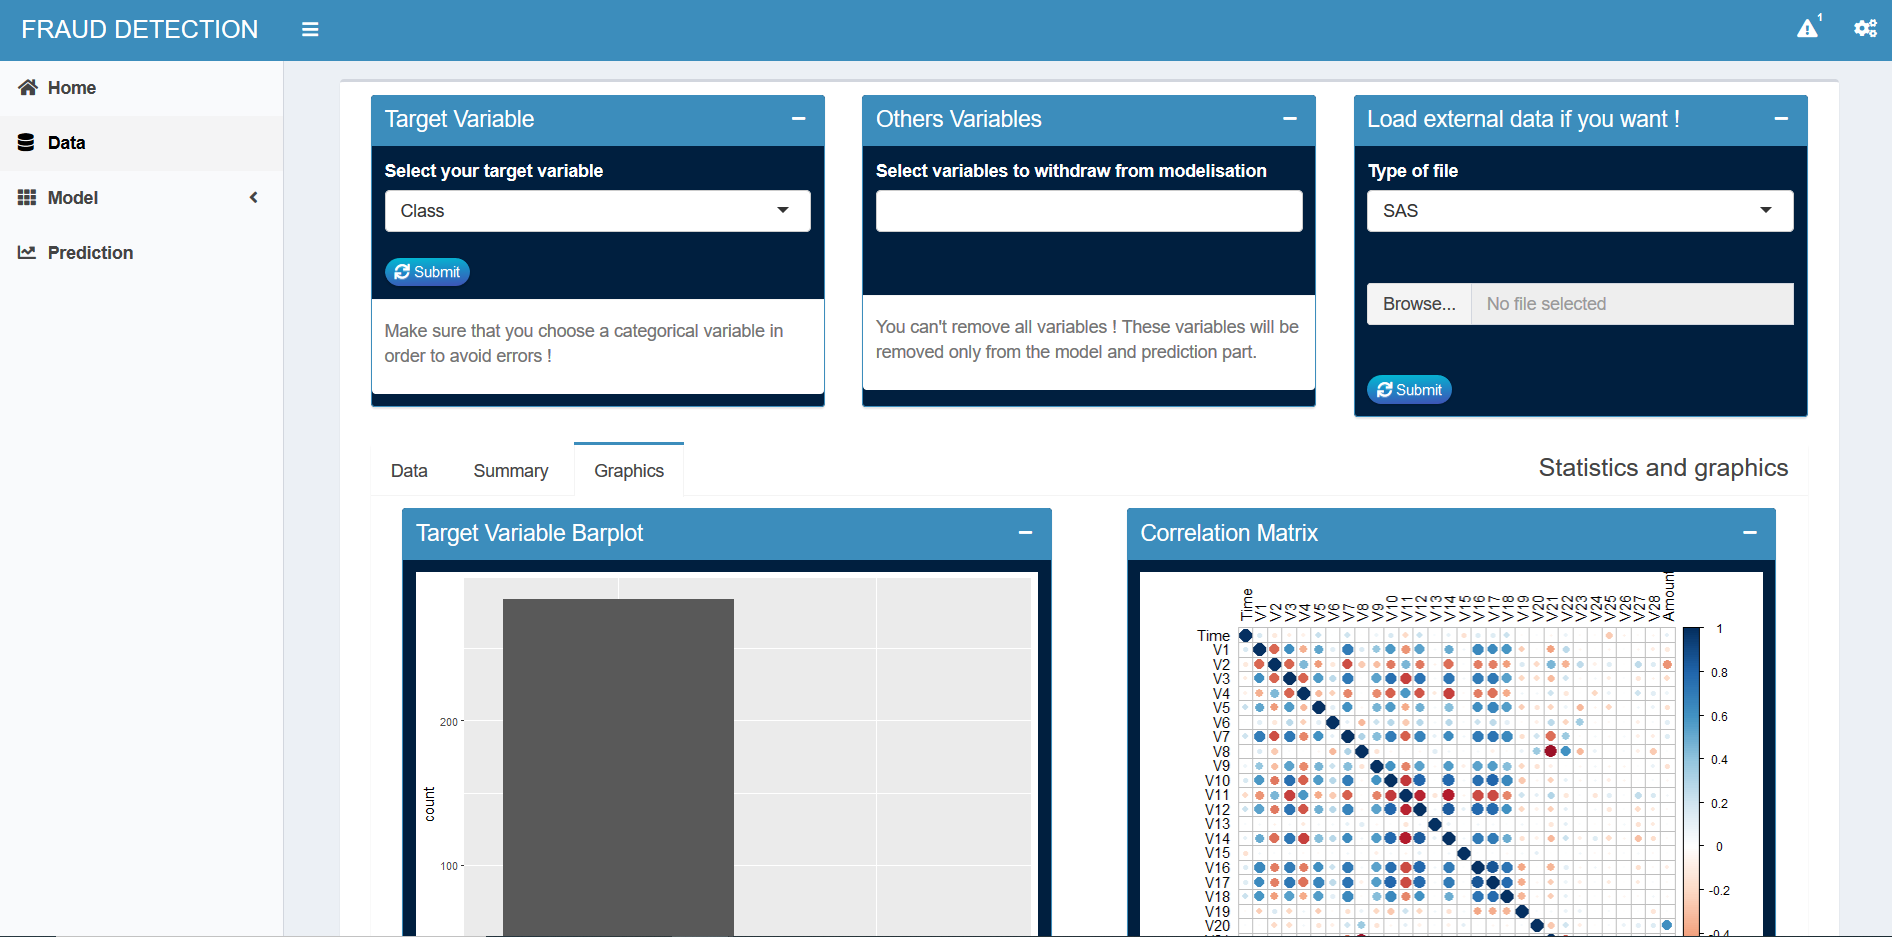
\includegraphics[width=12.00000cm]{https://raw.githubusercontent.com/Songui/Image/master/Capture3.PNG}
\caption{Data Step Interface}
\end{figure}

\section{Models part}\label{models-part}

In this part, you have three sub parts: Sampling, SVM method and
Benchmarking analysis. I remind you that we must follow the steps one by
one.

\begin{itemize}
\tightlist
\item
  \emph{\textbf{Sampling}}
\end{itemize}

At this level, you can choose the method that you think is appropriate
for resampling. Then, click on the submit button, otherwise nothing will
happen.

\begin{itemize}
\tightlist
\item
  \emph{\textbf{SVM method}}
\end{itemize}

At this level, you have two parts. One concerns the general description
of the Support Vector Machine method (SVM) and the other its
implementation and performance.\\
At the implementation, you have to choose the differents values of
parameters that interest you to do it. The parameters have been
individually described when you hover over each of them to enhance your
understanding. We also add an article, which helped us in our parameters
choice decision. You can download it by clicking on
``\textbf{Hyper-parameters choices}''. At the end, please click on the
submit button to see the results of our implementation.\\
\emph{Given the size of our database, wait a few seconds before see our
results}.

\begin{itemize}
\tightlist
\item
  \emph{\textbf{Benchmarking analysis}}
\end{itemize}

At this step, you have to choose the method that interests you to make a
comparison of the SVM performance. Please, also choose the
classification threshold and do not forget to click on the submit
button.

\section{Prediction}\label{prediction}

All the previous steps allow you to come to the prediction step,
described by its name.\\
It is the model developed in svm which makes it possible. You can
manually enter the desired values for each explanatory variable and
click on the submit button to view the value of the forecast.


\end{document}
